\chapter{Fontes principais de dados espaciais}

\pagestyle{fancy}

Até pouco tempo atrás, toda informação manipulada em um SIG tinha origem em um mapa em papel, que precisava ser \emph{preparado} para se adaptar à natureza digital do SIG. O dado geográfico era obtido por meio da \textbf{digitalização} da cartografia, ou seja, a conversão dos dados impressos em formato digital compatível com SIG.

Como aplicação computacional, um SIG depende exclusivamente de dados digitais. Os dados geográficos digitais oferecem várias vantagens em relação aos analógicos, além do simples fato de poderem ser incorporados ao SIG. Entre essas vantagens destacam-se: facilidade de atualização, distribuição simplificada (especialmente com a Internet), menor espaço de armazenamento físico, facilidade e precisão de análise, e manutenção eficiente (o dado digital não se degrada, apenas seu suporte, o que permite sua replicação sem perda de qualidade).

Atualmente, as técnicas de aquisição de dados evoluíram e permitem criar dados diretamente integráveis em um SIG. Assim, distinguimos \textbf{fontes primárias} e \textbf{fontes secundárias} de dados.

As \textbf{fontes primárias} geram dados que, em sua forma original, já podem ser utilizados em SIG, enquanto as \textbf{fontes secundárias} produzem dados que precisam de adaptação antes de serem usados.

Neste capítulo, exploraremos as diversas fontes de dados utilizáveis em um SIG.

\section{Sensoriamento remoto}\index{Sensoriamento remoto}

Sensoriamento remoto é o \textbf{estudo e medição das características de um objeto sem contato físico direto}. Mede-se, geralmente, a radiação eletromagnética refletida ou emitida pelos objetos na superfície terrestre.

Um sistema de sensoriamento remoto é composto pelos elementos da Figura~\ref{Fig:Elementos_teledeteccion}:

\begin{figure}[!hbt]   
\centering
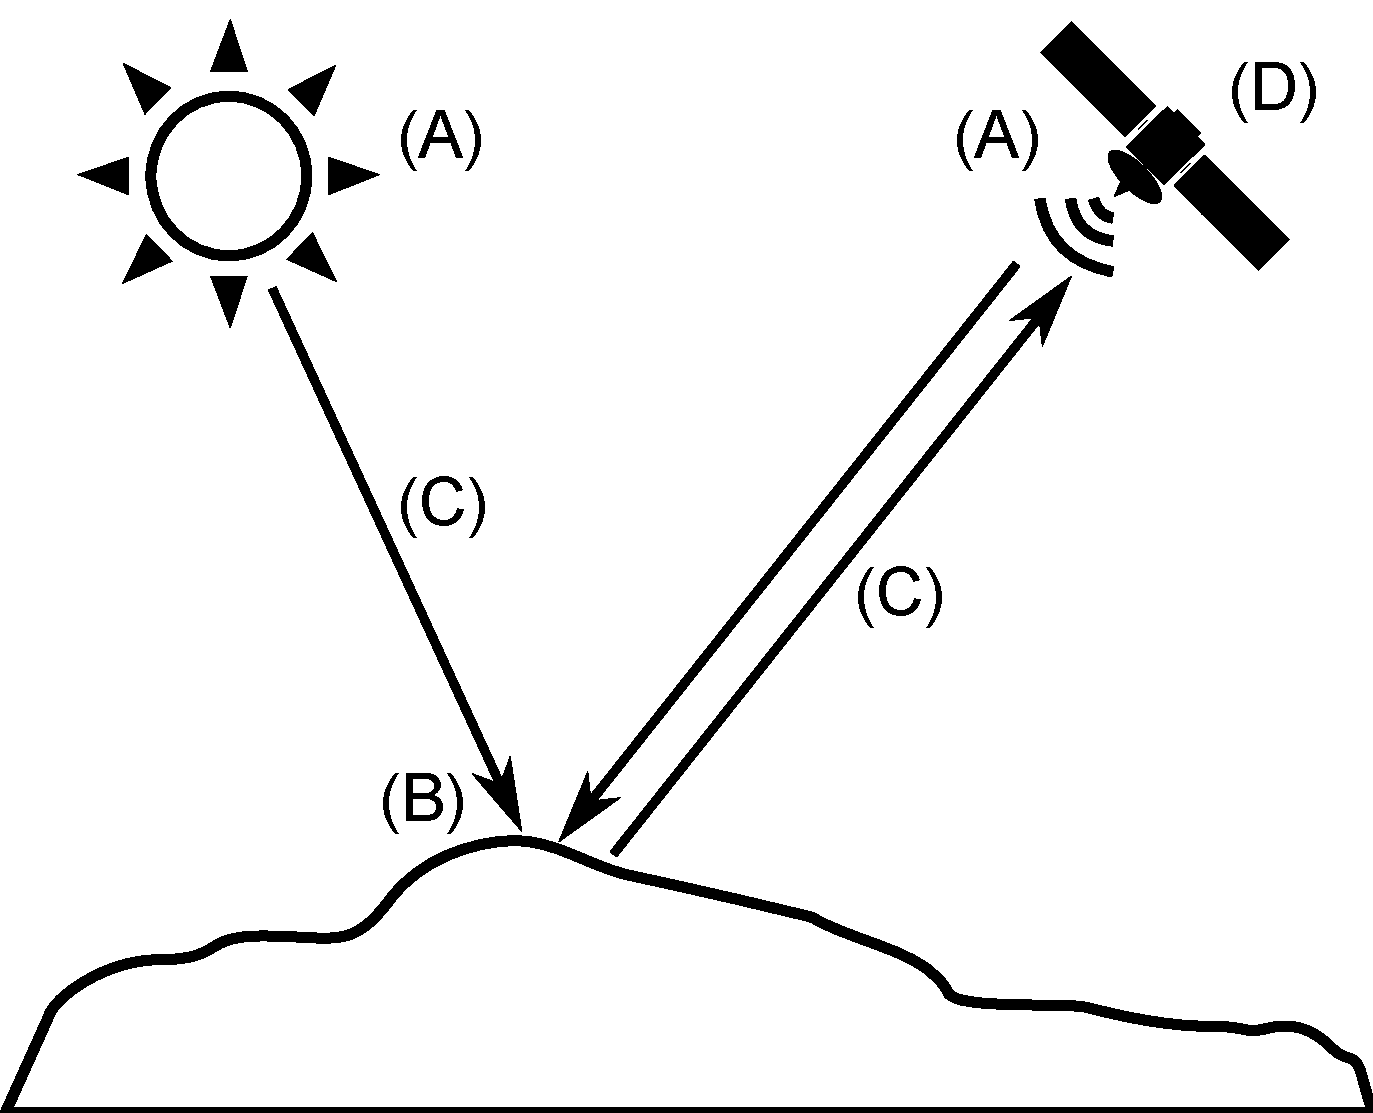
\includegraphics[width=.6\textwidth]{Fontes_dados/Elementos_teledeteccion.pdf}
\caption{\small Esquema de um sistema de sensoriamento remoto.}
\label{Fig:Elementos_teledeteccion} 
\end{figure}

\begin{itemize}
	\item \textbf{Fonte de radiação (A)}: natural ou artificial. A radiação interage com a superfície terrestre, sendo alterada por ela.
	\item \textbf{Objetos (B)}: refletem ou emitem radiação.
	\item \textbf{Atmosfera (C)}: atravessada pela radiação, podendo também alterá-la.
	\item \textbf{Receptor (D)}: capta a radiação refletida e gera uma imagem (camada raster), com valores de intensidade registrados em \textbf{Níveis Digitais} (geralmente entre 1 e 256).
\end{itemize}

A seguir, veremos detalhes desses elementos: fundamentos físicos (radiação e interação com a matéria) e análise dos receptores (sensores e plataformas).

\subsection{Fundamentos físicos}

A radiação eletromagnética resulta de alterações nos campos elétrico e magnético. Suas ondas propagam-se à velocidade da luz e são descritas por parâmetros como comprimento de onda e frequência. O conjunto dessas radiações compõe o \textbf{espectro eletromagnético}.

As principais interações dos objetos com a radiação são: \textbf{absorção, transmissão e reflexão}. Para o sensoriamento remoto, a \textbf{reflexão} é a mais relevante, pois é a radiação refletida que será captada para gerar imagens.

Cada objeto reflete radiações de diferentes comprimentos de onda de modo específico. Isso define sua \textbf{assinatura espectral}.

Imagens geradas possuem múltiplas bandas (valores por pixel), cada uma associada a uma faixa do espectro. Os Níveis Digitais em cada banda representam a intensidade da radiação naquela faixa específica.

\subsection{Sensores e plataformas}

Os principais elementos tecnológicos de um sistema de sensoriamento remoto são o \textbf{sensor} e a \textbf{plataforma}.

\begin{itemize}
\item \textbf{Sensores passivos} captam radiação natural (como a solar).
\item \textbf{Sensores ativos} emitem radiação (como radar e LiDAR) e captam sua reflexão.
\end{itemize}

O \textbf{LiDAR}, por exemplo, utiliza pulsos de laser e fornece dados sobre a \textbf{elevação}, sendo útil para mapear o relevo.

A \textbf{plataforma} é onde o sensor está instalado, podendo ser:
\begin{itemize}
\item \textbf{Atmosférica} (aviões) — oferecem flexibilidade de uso.
\item \textbf{Orbital} (satélites) — possuem órbitas definidas por parâmetros chamados de \textbf{parâmetros orbitais}.
\end{itemize}

Órbitas especiais incluem:
\begin{itemize}
\item \textbf{Geoestacionária} — acompanha a rotação da Terra.
\item \textbf{Heliossincrônica} — passa sempre pelo mesmo ponto à mesma hora solar.
\end{itemize}

\subsubsection{Resoluções}

Quatro tipos principais de resolução:

\begin{itemize}
\item \textbf{Espacial}: tamanho mínimo do objeto detectável (tamanho real do pixel).
\item \textbf{Espectral}: número e largura das bandas no espectro.
\item \textbf{Radiométrica}: profundidade dos Níveis Digitais (detalhe de intensidade).
\item \textbf{Temporal}: tempo entre duas aquisições de uma mesma área.
\end{itemize}

Nenhum sensor possui alta resolução em todos os aspectos. A escolha da imagem depende da aplicação.

\subsection{Fotogrametria}

Técnica que mede e define forma, dimensão e posição de objetos a partir de imagens, em especial \textbf{fotografias aéreas}. Utiliza \textbf{pares estereoscópicos} para criar \textbf{restituições 3D} do terreno.

Com imagens de satélite, pares são obtidos variando-se o \textbf{ângulo de visão} do sensor na mesma passagem.

Modalidades:
\begin{itemize}
\item \textbf{Analógica}
\item \textbf{Analítica}
\item \textbf{Digital} — base dos SIG.
\end{itemize}

Requer uma \textbf{estação fotogramétrica} digital com visualização estereoscópica, podendo incluir periféricos como \textbf{mouse 3D}.

\section{Cartografia impressa e digitalização}

Cartografia em papel (mapas, fotos antigas) precisa ser digitalizada para uso em SIG.

\begin{itemize}
\item \textbf{Raster}: via escaneamento.
\item \textbf{Vetorial}: exige registro geográfico, digitalização da geometria e dos atributos.
\end{itemize}

Digitalização pode ser:
\begin{itemize}
\item \textbf{Manual} — operador desenha entidades.
\item \textbf{Automática} — processo automatizado.
\end{itemize}

Dispositivos:

\begin{itemize}
\item \textbf{Tablet digitalizador}
\item \textbf{Editor SIG com mouse}
\end{itemize}

\textbf{Vectorização} é a digitalização automática para criar camadas vetoriais. A qualidade depende da preparação do documento.

Também é possível criar camadas a partir de \textbf{dados tabulares com coordenadas} (\textbf{geocodificação}). Se digitais, podem vir em planilhas, arquivos de texto, ou anexos de fotos (\emph{geotagging}).

\subsection{Qualidade da digitalização}

Erros podem surgir no processo, inclusive devido à fonte original (mapa degradado, linhas apagadas etc.). A Figura~\ref{Fig:Imprecisiones_digitalizacion} mostra exemplos.

\begin{figure}[!hbt]   
\centering
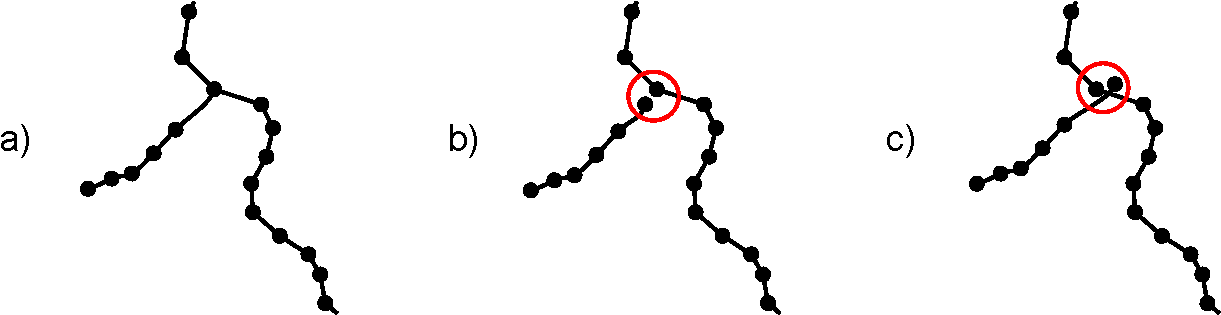
\includegraphics[width=\textwidth]{Fontes_dados/Imprecisiones_digitalizacion.pdf}
\caption{\small Erros na digitalização. a) Correto, b) e c) com nós desconectados.}
\label{Fig:Imprecisiones_digitalizacion} 
\end{figure}

SIGs modernos oferecem recursos de \textbf{snapping} e validação topológica para corrigir imprecisões durante a digitalização.

\section{GPS}

\textbf{Sistemas Globais de Navegação por Satélite (GNSS)} permitem determinar a posição de qualquer ponto na Terra com precisão de poucos metros.

O mais popular é o \textbf{GPS}, com 24 satélites operacionais. Usa \textbf{triangulação} e o datum \textbf{WGS84}.

Erros podem vir de:
\begin{itemize}
\item posição dos satélites,
\item reflexão do sinal,
\item interferência atmosférica,
\item imprecisão dos relógios.
\end{itemize}

\textbf{GPS diferencial} melhora a precisão usando um receptor fixo como referência. Isso permite alcançar:
\begin{itemize}
\item \textbf{2 m de precisão com correção}
\item \textbf{10–20 m sem correção}
\end{itemize}

Tipos de GPS:
\begin{itemize}
\item \textbf{Portátil} — para uso geral.
\item \textbf{Topográfico} — maior precisão e uso profissional.
\end{itemize}

Elementos coletados:
\begin{itemize}
\item \textbf{Waypoint} — ponto único.
\item \textbf{Track} — percurso contínuo.
\item \textbf{Route} — sequência de \emph{waypoints}.
\end{itemize}

\section{Informação Geográfica Voluntária (VGI)}

A \textbf{VGI} é a criação, gestão e compartilhamento de dados espaciais voluntários por usuários da Internet. Isso representa um \textbf{paradigma social e participativo}, rompendo com o monopólio estatal da cartografia.

Exemplo principal: \textbf{OpenStreetMap} (OSM).

Conceitos-chave:
\begin{itemize}
\item \textbf{Democratização da cartografia}
\item Cidadãos como \textbf{sensores ativos}
\item Redução do "mistério" da produção cartográfica
\end{itemize}

\section{Metadados}

\textbf{Metadados} são \textbf{dados sobre os dados}. Eles explicam, contextualizam e viabilizam o uso correto das informações geográficas.

Importância:
\begin{itemize}
\item Avaliar adequação dos dados.
\item Evitar uso indevido.
\item Facilitar busca, localização e catalogação.
\end{itemize}

Devem conter:
\begin{itemize}
\item \textbf{Identificação}
\item \textbf{Qualidade e linhagem dos dados}
\item \textbf{Componentes espaciais e temáticos}
\item \textbf{Distribuição e licenciamento}
\end{itemize}

Metadados podem ser:
\begin{itemize}
\item \textbf{Gerados na origem}
\item \textbf{Acrescentados depois} por distribuidores ou usuários
\end{itemize}

Formato:
\begin{itemize}
\item \textbf{Arquivos separados}
\item \textbf{Entradas em banco de dados}
\end{itemize}

\pagestyle{empty}
